\section{Methods}

\subsection*{The data}

As the goal of this study is to compare some forecasts on many different pandemics, a large set of synthetic pandemics need to be generated, with a particular attention on the diversity of these pandemics. 

\subsubsection{Covasim}

To generate the pandemics,  Covasim \cite{kerr2021covasim}, a python librairy that can simulate the evolution of a pandemic was used. 
Covasim is an agent-based model that can simulate many different pandemics and has a high diversity of outputs. 
This model takes as an input many parameters such as the population type, the population size, the age repartition... and outputs a complete description of the pandemic, with real-time values of each relevant information, such as the number of severe, of asymptomatic... but also physical values such as the value of the reproduction number. 
Covasim enables to generate a huge diversity of pandemics, thanks to the plurality of parameters that can be given as the input of the model, but also with interventions that can be planned by the users. 
These interventions can help to assess the impact of a vaccination campaign, with changes in the probability transmission. 

\subsubsection{First pandemics}

For the implementation and the first test of the models, two pandemics were generated. 
The first one focusing on the new deaths count and the second one focusing on the number of hospitalized count. 
Those pandemics will be referred to as pandemic 1 and pandemic 2. 

\begin{table}[htbp]
    \centering
    \caption{Table of the parameters used to simulate the first two pandemics.}
    \label{tab:parameters_covasim}
    \begin{tabular}{|c|c|c|}
        \hline
        \textbf{Parameter} & \textbf{Pandemic 1} & \textbf{ Pandemic 2} \\
        \hline
        start day 1 &2020-03-02 & 2020-03-02\\
        \hline

        end day  &2020-07-01 & 2021-01-01\\
        \hline

        Population size &1000000&1000000\\
        \hline

        Interventions & interventions1 & interventions2\\
        \hline

        population type& hybrid & hybrid\\

        \hline

        $\beta$ initial &0.015 & 0.015\\
        \hline

        location & Sweden & Sweden \\
        \hline

        n infected initial &20&100\\
        \hline
    \end{tabular}
\end{table}



The parameters used to generate these pandemics are described in the table \ref{tab:parameters_covasim} 
The parameters that are not specified are the default parameters of the Covasim librairy. 


\begin{figure}
    \centering
    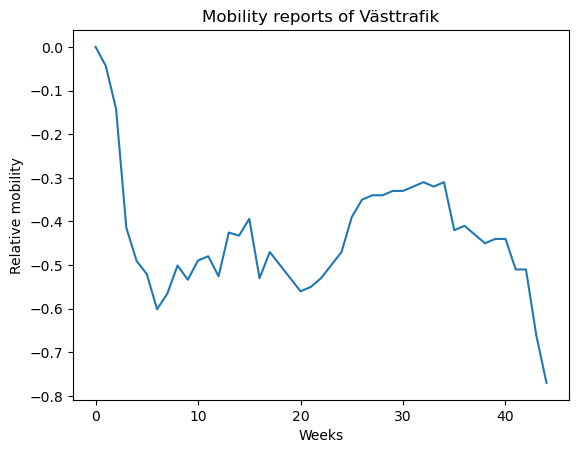
\includegraphics[width=0.5\textwidth]{figures/mobility_reports.png}
    \caption{Mobility reports from Västtrafik.}
    \label{fig:mobility_reports}
\end{figure}


The different interventions were based on mobility reports from Västtrafik (Fig.\ref{fig:mobility_reports}), the public transport company of the city of Gothenburg, which were reported during the Covid 19 pandemic and has been retrieved in \cite{gerlee2021predicting}.
These interventions correspond to 53 relative weekly variations of the mobility, with a reference value of 1 for the first week of the report, which correspond to the 9-th week of 2020. 


\subsubsection{Generating diverse pandemics}
\label{sec:generating_divserse_pandemics}
In order to evaluate the performances of our models on a wide range of pandemics, a training set of pandemics was generated. 
A huge diversity of pandemics is needed to determine which model is the more consistent.
It is so relevant to identify the key parameters that generate this diversity.
As Covasim has a very huge set of inputs parameters, a first subset of key parameters was identified: the spread parameters and the severity parameters. 
The severity parameters are the 4 parameters that correspond to the probability for an agent to get from a compartment to another. 
The spread parameters are 9 parameters that represent the distribution of probability of the time spend by an agent in a compartment (such as infected, crictical...) once he entered it. 
This distribution is a log-normal distribution, but the spread-parameters correspond to the mean of this log-normal distribution
All the parameters have a default value of 1, which correspond to keeping the reference value. 
We decided to select 4 parameters and to make them vary in $[0.5, 1, 2]$, leading to a set of 81 pandemics. 
To select the 4 parameters that generated the most diversity, different diversity metrics were computed. 

Let $Y_1$ ,  $Y_2 \in \mathbb{R}^n$  be two time series of $n$ days representing the number of hospitalized in two pandemics.  

Let :  \\

$
\begin{aligned}
    &\mathcal{L}_1(Y_1, Y_2) = \| Y_1 - Y_2 \|_{L_1}  \\
    &\mathcal{L}_2(Y_1, Y_2) = \| (\frac{max(Y_1)}{max(Y_2)} ;\frac{max(Y_1')}{max(Y_2')} ; \frac{max(Y_1'')}{max(Y_2'')} , \| \tilde{Y_1} - \tilde{Y_2} \|_{L_1}, \| \tilde{Y_1'} - \tilde{Y_2'} \|_{L_1} , \| \tilde{Y_1''} - \tilde{Y_2''} \|_{L_1} ) \|_{L_2} \\
    &\quad \quad\quad\quad\quad \quad\quad\quad \quad\quad\quad\quad \quad\quad\quad\quad \quad\quad\quad\quad \quad\quad\quad\text{ with }Y' \text{ and } Y'' \text{the first and second derivatives of} Y\\
    &\mathcal{L}_3 = \mathcal{W}(\tilde{Y_1} - \tilde{Y_2}) \text{, with }\mathcal{W} \text{ the Wasserstein distance.} \\
    &\mathcal{L}_4(Y_1, Y_2) = \| (\frac{max(Y_1)}{max(Y_2)} ;\frac{max(Y_1')}{max(Y_2')} ; \frac{max(Y_1'')}{max(Y_2'')} , \mathcal{W} (\tilde{Y_1} - \tilde{Y_2} ),\mathcal{W} ( \tilde{Y_1'} - \tilde{Y_2'} ) , \mathcal{W} (\tilde{Y_1''} - \tilde{Y_2''} ) ) \|_{L_2} \\
    &\quad \quad\quad\quad\quad \quad\quad\quad \quad\quad\quad\quad \quad\quad\quad\quad \quad\quad\quad\quad \quad\quad\quad\text{ with }Y' \text{ and } Y'' \text{the first and second derivatives of} Y\\[1cm]
\end{aligned}
$

It can be noted that $\mathcal{L}_2$ looks like the Sobolev norm  $\| \tilde{Y_1}  - \tilde{Y_2} \|_{W^{2, 1}} $ with squared terms and with additionary terms taking into account the amplitude. 

To determine which measure to use, we generated 14 pandemics. 
Each pandemic but the last one has default parameters except one of them which was doubled. 
The last pandemic has only default parameters. 

For each norm $\mathcal{L}_k$, we determined $S$,  the subset of 4 pandemics that maximized the following quantity:\\

\[ \sum_{i, j \in S, i \neq j} \mathcal{L}_k(Y_i, Y_j) \]

\begin{figure}
    \centering
    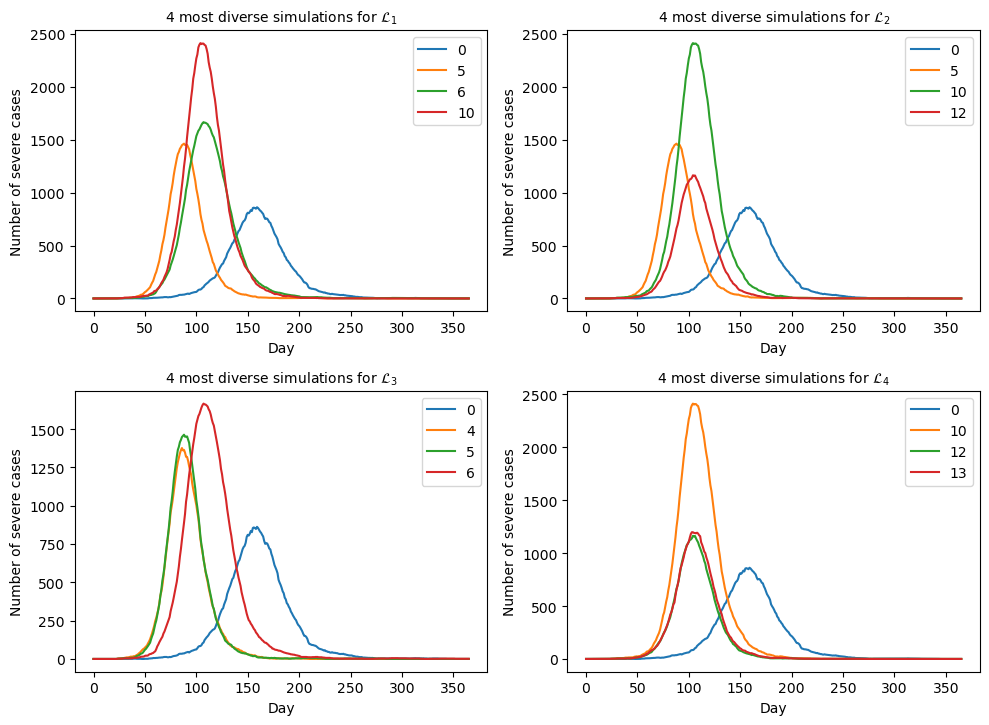
\includegraphics[width=0.8\textwidth]{figures/most_different_pandemics.png}
    \caption{4 most diverse pandemics according to each norm.}
    \label{fig:diversity_pandemics}
\end{figure}


The 4 most divers pandemics accorded to each norm are shown in the figure \ref{fig:diversity_pandemics}.
We decided according to this figure, that $\mathcal{L}_2$ norm was the most relevant to determine the diversity of the pandemics.
But, keeping the parameters \texttt{[0, 5, 10, 12]} would not be accurate, as the parameters were changed independantly, and the diversity did not take into account the correlation between some of them. 

Finding the parameters that maximise the $\mathcal{L}_2$ diversity is equivalent to solve the following problem : \\

$ S_{opt} = \underset{S' \subset S , \vert S' \vert =4 }{argmax} \mathcal{L}(S')$, with $ \mathcal{L}(S')= \sum_{s, t \in \mathcal{P}_g(S') , s \neq t }{\mathcal{L}_2(s,t)}$, and  $\mathcal{P}_{g}(S')$ the set of the 81 pandemics generated with the 4 parameters of $S'$

However, generating a pandemic with \texttt{Covasim} is time consuming, and it is not possible to compute the diversity of each set of 4 parameters $S'$ included in $S$.\\[1cm]


A MCMC algorithm \cite*{diaconis2009markov} was then implemented, to perform a clever grid search on the different subsets $S' \subset S $ of parameters.
The MCMC algorithm is a method which is used to sample from a distribution that can't be directly sampled. 
The main idea is to construct a Markov Chain whose stationary distribution is the objective distribution.

Let $\mathcal{S} = \{ S'\subset S ;  \vert S' \vert = 4 \}$ be the support of the target distribution, which is, in our case, the set of all the 715 combinations of the 4 parameters among the 13 different possible, and let $\pi$ be the target distribution on $\mathcal{S}$.
$\forall s \in \mathcal{S}, \pi(s) = \frac{\mathcal{L}(s)}{\sum_{s \in \mathcal{S}}  \mathcal{L}(s)} $. $\pi$ is not directly computable as it is too time consuming to compute the denominator.


For each $s = [a, b, c, d] \in \mathcal{S}$, let $ne(s)$ be the set of the neighbourghs of $s$, i.e the set of all the elements of $\mathcal{S}$ who have only one parameter different from $s$. 
For instance, $[0, 3, 9, 12] \in ne([0, 3, 10, 12])$, but $[0, 3, 9, 12] \notin ne([0, 3, 8, 10])$.\\

Let $U_n$ be a sequence of independent uniform random variables on $[0, 1]$ and $\forall s \in \mathcal{S}$, let $U_{n}^{ne(s)}$ be a sequence of independant uniform random variables on $ne(s)$ .
Let $s_0 \in \mathcal{S}$ and let  $S_n$ be the random sequence defined as follow : \\


\[
 \left\{
    \begin{aligned}
        & S_0 = s_0 \\
        & \forall n \in \mathbb{N}, \alpha_n = \frac{\mathcal{L}(U_{n}^{ne(S_n)})}{\mathcal{L}(\mathcal{S}_n)} \\
        & \forall n \in \mathbb{N}, S_{n+1} = U_{n}^{ne(S_n)} \mathbb{1}_{\{U_n < \alpha_n\}} + X_n \mathbb{1}_{\{U_n > \alpha_n\}}
\end{aligned}
\right.
\]
\\[0.5cm]

As $S_{n+1}$ is a function of $S_n$ and of other independant random variables, the sequence $S_n$ is a homogenous Markov Chain.
This formula means that at each iteration, a neighbourgh of $S_n$ is uniformly selected among all the neighbourghs of $S_n$ (it is $U_n^{ne(S_n)}$)
The Markov Chain moves to this neighbourgh if the value of  $\mathcal{L}(U_n^{ne(S_n)})$ is higher than the value of the function $\mathcal{L}(S_n)$ at the current state.
If the new value of $\mathcal{L}$ is smaller, the markov chain moves with a probability that is equal to the ratio of the two values.
This way of moving on the different subsets prevents to be stucked in a local maxima but avoids exploring dummies areas, in which the diversity is very small. \\

The transition matrix of this Markov Chain is the following: 
\[
K(s, s'): \left\{
\begin{aligned}
& 0 \text{ if } s' \notin ne(s) \text{ and } s' \neq s   \\
& \frac{1}{Card(ne(s))} = \frac{1}{36} \text{ if } s' \in ne(s) \text{ and } \frac{\mathcal{L}(s')}{\mathcal{L}(s)} > 1 \text{ and } s' \neq s \\
& \frac{1}{36} \times \frac{\mathcal{L}(s')}{\mathcal{L}(s)} \text{ if } s' \in ne(s) \text{ and } \frac{\mathcal{L}(s')}{\mathcal{L}(s)} \leq 1  \text{ and } s' \neq s  \\
& 1 - \sum_{s' \in \mathcal{S}, s' \neq s}K(s, s') \text{ if } s' = s 
\end{aligned}
\right.
\]
\\[0.3cm]

Let $(s, s') \in \mathcal{S}^2$. Let us suppose that $ s' \neq s$, that  $s' \in ne(s)$, and that $\mathcal{L}(s) < \mathcal{L}(s')$ (the other case is symmetric). \\[0.15cm]
$
\begin{aligned}
    \pi(s)K(s, s') &=  \frac{\mathcal{L}(s)}{\sum_{s \in \mathcal{S}} \mathcal{L}(s)} \times \frac{1}{36} \quad \text{as} \ \mathcal{L}(s) < \mathcal{L}(s') \\
    &=  \frac{\mathcal{L}(s)}{\sum_{s \in \mathcal{S}} \mathcal{L}(s)} \times \frac{1}{36} \times \frac{\mathcal{L}(s')}{\mathcal{L}(s')} \\
    &=  \frac{\mathcal{L}(s')}{\sum_{s \in \mathcal{S}} \mathcal{L}(s)} \times \frac{1}{36} \times \frac{\mathcal{L}(s)}{\mathcal{L}(s')} \\
    &= \pi(s')K(s', s)\\[0.3cm]
\end{aligned}
$
Indeed, each subset $s$ has 36 neighbourgh, as there are 13 parameters and one can replace each parameter of $s$ by any of the 9 others. \\
Thus, $\pi$ is \textbf{reversible} for $K$.\\
Let $(s, s') \in \mathcal{S}^2$. Let us note $(a, b, c, d)$ and $(a', b', c', d')$ the elements of $s$ and $s'$.
We note : \\
$s_1 = [a', b, c, d]$\\
$ s_2 = [a', b', c, d]$ \\
$s_3 = [a', b', c', d]$ \\


$
\begin{aligned}
    \mathbb{P}(S_{n+4}=s'\vert S_n = s ) & \geqslant \mathbb{P}(S_{n+4} = s' \cap  S_{n+3}= s_3 \cap S_{n+2} = s_2 \cap S_{n+1} = s_1 \vert S_n = s) \\
    & \geqslant \mathbb{P}(S_{n+4} = s' \vert S_{n+3} = s_3 \cap S_{n+2} = s_2 \cap S_{n+1} = s_1 \cap S_n = s) \\
    & \quad\quad\quad\quad \times \mathbb{P}( S_{n+3} = s_3 \cap S_{n+2} = s_2 \cap S_{n+1} = s_1 \vert S_n = s) \text{  (Baye' s Formula)}\\
    & \geqslant \mathbb{P}(S_{n+4} = s' \vert S_{n+3} = s_3) \times \mathbb{P}( S_{n+3} = s_3 \vert S_{n+2} = s_2 \cap S_{n+1} = s_1 \cap S_n = s) \\
    & \quad\quad\quad\quad \times \mathbb{P}( S_{n+2} = s_2 \cap S_{n+1} = s_1 \vert S_n = s ) \text{ (by Markov's property)}\\
    & \vdots \\
    & \geqslant \mathbb{P}(S_{n+4} = s' \vert S_{n+3} = s_3) \times \mathbb{P}( S_{n+3} = s_3 \vert S_{n+2} = s_2) \times \mathbb{P}( S_{n+2} = s_2 \vert S_{n+1} = s_1) \\
    & \quad\quad\quad\quad \times \mathbb{P}( S_{n+1} = s_1 \vert S_n = s ) \text{ (by Markov's property)}\\
    & \geqslant (\frac{1}{36})^4 \times min (1, \frac{\mathcal{L}(s')}{\mathcal{L}(s)}) \times min (1, \frac{\mathcal{L}(s_3)}{\mathcal{L}(s_2)}) \times min (1, \frac{\mathcal{L}(s_2)}{\mathcal{L}(s_1)}) \times min (1, \frac{\mathcal{L}(s_1)}{\mathcal{L}(s)})  \\
    & > 0 \\
\end{aligned}
$

Thus, $S_n$ is \textbf{irreducible}.\\

A Markov chain of transition matrix $P$ on the support $\mathcal{S}$ is said to be aperiodic if: \\
$\forall s \in \mathcal{S}, \forall s' \in \mathcal{S}, \exists N \in \mathbb{N}, \text{ s.t } \forall n > N, P(s, s')^n >0 $ \cite[text]{bodineau2015modelisation}\\

First, note that $\forall s \in \mathcal{S}$,  $s$ is a local minimum (i.e if $\forall s' \in ne(s), \mathcal{L}(s') > \mathcal{L}(s) $) if and only if $K(s,s)=0$\\

Thus, if $s$ is not a local minimum, then $K(s, s)>0$. Moreover, $ \forall s \in \mathcal{S}, \forall s' \in ne(s)$, if $s\neq s'$, then $K(s, s') \neq 0 $\\[0.3cm]
Let $(s, s')  \in \mathcal{S}^2$. \\

\begin{itemize}
    \item If $s'$ is not a local minimum, \\
     $\forall n >4, \mathbb{P}(S_{n} = s' \vert S_0 = s) \geqslant \mathbb{P}(S_{4} = s' \vert S_0 = s) \times K(s', s')^{n-4} > 0 $ \\
    \item If $s'$ is a local minimum,  $\forall s^* \in ne(s')$, $s^*$ is not a local minimum and $K(s^*, s^*) \neq 0$. \\
    $\forall n>5$, $\mathbb{P}(S_n = s' \vert S_0 = s )   \geqslant \mathbb{P}(S_3=s^* \vert S_0 = s ) \times K(s^*, s^*)^{n-4} \times K(s^*, s') >0 $\\
    
\end{itemize}

Thus $S_n$ is an \textbf{aperiodic} Markov Chain.\\


Finally, according to the \textbf{Theorem 5.5 } from \cite*{bodineau2015modelisation}, as $S_n$ is irreductible and aperiodic, as $\pi$ is the stationary distribution, and as $\mathcal{S}$ is countable, $S_n$ converges in distribution to $\pi$.


The most probable set that will be sampled by $S_n$ is so the one that maximises the diversity.
We implemented this MCMC algorithm to maximise $\mathcal{L}_2$ on $\mathcal{S}$ . 
After 200 iterations, the set of parameters that maximised the diversity was \texttt{[0, 5, 10, 12]}. 
A new maxima was found at \texttt{[2, 4, 9, 10] }, which correspond to the parameters \texttt{[sym2sev, asym2rec, rel\_symp\_prob, rel\_severe\_prob]}. 
The $\mathcal{L}_2$- diversity increased from 62353 to 93553. \\

To create the most diverse set possible, we also created 4 different mobilities reports \ref{fig:mobilities}, corresponding to constant mobility, annual variations, lockdown scenario and the reports from Vasträffik from \cite{gerlee2021predicting}. 
\begin{figure}
    \centering
    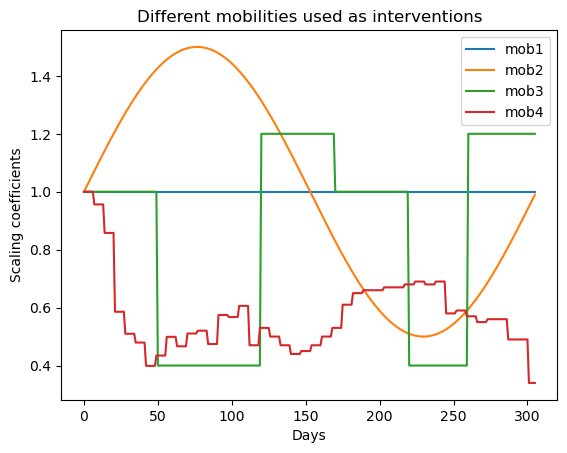
\includegraphics[width=0.8\textwidth]{figures/mobilities.png}
    \caption{Mobility reports.}
    \label{fig:mobilities}
\end{figure}
These time-varying mobilities enabled us to model more complex behaviours of the pandemics. 
We finally modelled 324 pandemics. 
Indeed each of the 4 parameters was scaled among 3 values : \texttt{[0.5, 1, 2]} and the 4 mobilities reports were used.


\subsection{The models}

In this study, we define a model ${h}_{\theta }$ as a function ${h}$  defined on $ \mathbb{N}$, with parameters $\theta$ and trained on the data $\mathcal{D}$.
In the training phase, $\hat{\theta}$,  an estimator of $\theta$ is computed form $\mathcal{D}$, and used for the prediction.  
We elaborated two types of models: the first type correspond to models which are only trained on the time series we want it to predict (the number of hospitalized in our case), and the second type of models are trained on the time series we want to predict, but also on other time series that can be relevant to predict the number of hospitalized (the mobility and the number of infected). 
All of these models were implemented in Python, and are available on the github repository provided with this article (\ref{github-link}).
During the training or predicting phase, the computation sometimes fail (for instance, when the matrix is non-inversible for the linear regression model). 
The model then outputs the value of the mving average model, which can be interpreted as a naive output when the computation fails. \\
\textbf{Task of a model}: \\

Each model ${h}$ is given : 

\begin{enumerate}
    \item A training set $\mathcal{D}$
    \item A reach of prediction $r$
    \item A confidence threshold $\alpha$
\end{enumerate}
And outputs: 

\begin{enumerate}
    \item A prediction $\hat{Y}_r$
    \item A $(1-\alpha)$ confidence interval on the prediction, $I_{\alpha, r}$
\end{enumerate}

The model will train on the data $\mathcal{D}$ to compute $\hat{\theta}$ the parameter estimator and the output $\hat{Y}_r = {h}_{\hat{\theta}}(r)$.


\subsubsection{The SIRH model}



\begin{figure}[h]
    \centering
    \begin{tikzpicture}[
        roundnode/.style={circle, draw=blue!60, fill=gray!5, very thick, minimum size=7mm},
        arrow/.style={-{Stealth[scale=1]}, thick},
        every node/.style={scale=2.0}
        ]

        % Nodes
        \node[roundnode]      (s)                     {S};
        \node[roundnode]      (i) [right=of s]        {I};
        \node[roundnode]      (h) [right=of i]        {H};
        \node[roundnode]      (r) [below=of i]        {R};

        % Arrows
        \draw[arrow] (s) -- (i) node[midway, above, font=\footnotesize] {$\beta$};
        \draw[arrow] (i) -- (h) node[midway, above, font=\footnotesize] {$h$};
        \draw[arrow] (i) -- (r) node[midway, left, font=\footnotesize] {$\gamma_i$};
        \draw[arrow] (h) -- (r) node[midway, right, font=\footnotesize] {$\gamma_h$};

    \end{tikzpicture}
    \caption{Scheme of the SIRH model}
    \label{fig:sirh}

    
\end{figure}

The SIRH model (\ref{fig:sirh}) is an extension of the classic compartemental SIR (Susceptible-Infectious-Recovered) model used to describe the spread of infectious diseases.
In the SIRH model, a fourth compartment, "H" for "Hospitalized," is added. 
Each compartment correspond to the number of person in the state of health of the compartment. 
The evolution of the number of person in each compartment is described by a system of ordinary differential equations: 

\begin{equation}
    \label{eq:sirh}
    \left\{
    \begin{aligned}
        &\frac{dS}{dt} = - \beta \frac{SI}{N} \\
        &\frac{dI}{dt} = \beta \frac{SI}{N} - \gamma_i I - h H \\
        &\frac{dR}{dt} = \gamma_i I + \gamma_h h \\
        &\frac{dH}{dt} = h I
    \end{aligned}
    \right.
\end{equation}

At $t=0$, the values of $(S_0, I_0, R_0, H_0)$ is fixed to $(10^6 -1, 1, 0, 0,) $. 
As the system of equation can't be directly solved, we use a Euler method to solve it : \\


\begin{equation}
    \left\{
    \begin{aligned}
        S_{t+dt}=S_t + dt \frac{dS}{dt}\\
        I_{t+dt}=I_t + dt \frac{dI}{dt}\\
        R_{t+dt}=R_t + dt \frac{dR}{dt}\\
        H_{t+dt}=H_t + dt \frac{dH}{dt}\\
    \end{aligned}
    \right.
\end{equation}


We chose to fix $dt=0.001$. 




To train this model, we minimize the least square between the curve of the number of hospitalized observed to the curve of the number of hospitalized of teh training data with respect to $\theta = (\beta, gamma_i, gamma_h, h)$. 
We implemented some variations of the model in which $\gamma_i$, $\gamma_h$ or both were fixed to the value $0.2$. 

TODO : add a table of which coefficient are constant or not sirh 1 = cst, cst/ sirh2 = cst, free / sirh3 = free , cst / sirh4 = free, free. 
In the prediction phase, a $r$ day SIRH simulation is launched, with the parameter $\hat{\theta}$ computed during the training phase. 
The initial value for $S$ and $I$ correspond to the last value of the fit of the training phase. 
The initial value for $H$ correspond to the last value of $\mathcal{D}$, the trainig data. 
The initial value of $R$ is fixed by the previous values as the equation $S_t + I_y + R_t + H_t = N$ is always true. 
The confidence interval of the prediction is computd thanks to a linearization and the use of the delta-method (see \ref{sec:ci})


A SIRH model of the second type was implemented. 
It has the same structure but uses the mobility data and the number of infected to be more precise. 
The idea is the same, but there are two differences : 
\begin{itemize}
    \item $\beta$ varies with the time as a linear combination of the mobility : $\beta_t = a + b \times m_t$ 
    \item The data is fitted to both the number of hospitalized and the number of infected. 
\end{itemize}
To write it more formally, let $H_\theta(t)$ and $I_\theta(t)$ be the number of hospitalized and infected at time $t$ in the SIRH model with parameters $\theta$.
Let $Y_{H, t}$ and $Y_{I, t}$ be the number of hospitalized and infected at time $t$ in the data.
We have :\\

$\hat{\theta} = \underset{\theta \in \mathbb{R}^5}{\operatorname{argmin}} \sum_{t=1}^{n} (\frac{H_\theta(t) - Y_{H, t}}{\underset{t \in \{1, ..., n \}}{max(Y_{H, t})}})^2 + (\frac{I_\theta(t) - Y_{I, t}}{\underset{t \in \{1, ..., n \}}{max(Y_{I, t})}})^2$\\

With $\theta = (a, c, \gamma_i, \gamma_h, h)$ and $m_t$ the mobility at time $t$.
The normalization factors enables to prevent the optimization to focus on the number of infected, which is bigger than the number of hospitalized. 
Once again, a variation of the SIRH model was implemented, in which the value of $\gamma_h$ and $\gamma_i$ is fixed to $0.2$. 



\subsubsection{ARIMA and VAR models} 

The ARIMA and VAR models are used for time-series forecasting and have outperformed many models in pandemic prediction (see \cite[text]{kufel2020arima} and \cite[text]{shang2021regional})
The $ARIMA(p, d, q)$ model is the sum of an $AR(p)$ and a $MA(q)$ model applied on the time series differenciated $d$ times. 
It follows the equation : \\
$Y_{t}^{d}=\alpha+\sum_{i=1}^{p}\beta_{t-i}\,Y_{t-i}^{d}\,+\,\sum_{j=1}^{q}\phi_{t-j}\,\epsilon_{t-j} \label{eq:arima}$\\ 
where $Y_{t}^{d}$ is the time series at time $t$, $d$ is the order of the differencing, $\alpha$ is a constant, $p$ is the order of the autoregressive part, $q$ is the order of the moving average part and $\epsilon_{t-j}$ is the difference between the prediction of the model and the real value at time $t-j$.\\
The coefficient are estimated through maximum likelihood estimation. 
This method is implemented in the \texttt{statsmodels} library, which directly provide prediction and confidence intervals.
We realized a grid search on a single pandemic to identify the combinaition of parameters that would optimize the prediction accuracy. 
We found an optimal value for $p= 3, d=0, q=3$. 

The VAR model is a multi-dimensional $AR$ model, in which different variable are predicted. 
It so corresponds to a second type model. 
This model exploits the correlation between variables. 
The value of the parameters of a VAR have physical sense and can be interpreted to find correlations between variables. 
Let $Y_{1,t}, ..., Y_{k,t}$ be the times series (in our case, $k=3$ and they correspond to the number of hospitalized, the number of infected and the mobility data).


\[
VAR(p) : 
\begin{pmatrix}
Y_{1,t} \\
Y_{2,t} \\
\vdots \\
Y_{k,t}
\end{pmatrix}
=
\begin{pmatrix}
c_1 \\
c_2 \\
\vdots \\
c_k
\end{pmatrix}
+
\begin{pmatrix}
\phi_{11,1} & \phi_{12,1} & \cdots & \phi_{1k,1} \\
\phi_{21,1} & \phi_{22,1} & \cdots & \phi_{2k,1} \\
\vdots & \vdots & \ddots & \vdots \\
\phi_{k1,1} & \phi_{k2,1} & \cdots & \phi_{kk,1}
\end{pmatrix}
\begin{pmatrix}
Y_{1,t-1} \\
Y_{2,t-1} \\
\vdots \\
Y_{k,t-1}
\end{pmatrix} 
+ \cdots + 
\begin{pmatrix}
\phi_{11,p} & \phi_{12,p} & \cdots & \phi_{1k,p} \\
\phi_{21,p} & \phi_{22,p} & \cdots & \phi_{2k,p} \\
\vdots & \vdots & \ddots & \vdots \\
\phi_{k1,p} & \phi_{k2,p} & \cdots & \phi_{kk,p}
\end{pmatrix}
\begin{pmatrix}
Y_{1,t-p} \\
Y_{2,t-p} \\
\vdots \\
Y_{k,t-p}
\end{pmatrix}
+
\begin{pmatrix}
\epsilon_{1,t} \\
\epsilon_{2,t} \\
\vdots \\
\epsilon_{k,t}
\end{pmatrix}
\]


Again, the $\phi_{i,j,k}$ and  $c_i$ are estimated through maximum likelihood estimation with the \texttt{statsmodel} librairy. 
The confidence intervals are also directy provided by the librairy.
\subsubsection{The moving average model}

A mere moving average model was also implemented. 
It returns a constant prediction that correspond to the mean of the 7 past days. 
The confidence intervals are computed by assuming that the predictions follow a normal distribution of variance equal to the variance of the 7 past data-points; 
This model is used as a baseline.
A model that does not manage to outperform the moving average model would not be relevant.

\subsubsection{Exponential regression}

An exponential regression model was implemented.
It correspond to fitting the data of the number of hospitalized ($Y_t$) to the function $E_{a, b, c}(t) = a \times e^{b t} +c$.
The value of $\theta = (a, b, c)$ is computed through a least square method.
The confidence interval on the prediction is estimated with the same method as SIRH (see \ref{sec:ci}). 

An exponential regression of the second type was also implemented: \\
The data of the number of hospitalized is fitted to the function $E_{a, b, c, d, e}(t) = a \times e^{b m_{t-i} + c  t + d inf_{t-j} }+e$.
The value of $\theta = (a, b, c, d, e)$ is computed through a least square method.
The optimal value of the time lag $i$ and $j$ is optimized during the training phase through a grid search among all the values between 0 and 14. 
The confidence interval on the prediction is estimated with the same method as SIRH (see \ref{sec:ci}). 

\subsubsection{Machine learning models}
\label{sec:mlmodels}

In order to implement machine learning regressor, we converted the time-series $Y_{t, t \in {1, \vdots n}}$ in a training set $(X_i, Y_i)$ such that : \\
$\forall i \in \{1, ..., n\}, X_i = (Y_{i-1}, Y_{i-2}, ..., Y_{i-20})$.\\

We then trained and optimized both regressors : the linear and the bayesain regression, which were the only one that did not output absurd results on the \texttt{scikit-learn} models among : linear regression, bayesian regression, Ridge, Gradient boosting regressor, Random Forest regressor, Bayesain Ridge and SVR. 
The confidence interval for the linear regression prediction was computed as follow : \\
Let us suppose that the data follows a linear regression model : $Y = X\beta + \epsilon$, with $Y \in \mathbb{R}^n$, $X \in \mathbb{R}^{n \times d}$, $\beta \in \mathbb{R}^d$ and $\epsilon \sim \mathcal{N}(0, \sigma^2)$.
The least square estimator of $\beta$ is $\hat{\beta} = (X^T X)^{-1} X^T Y$.
If we have new data $\tilde{X} \in \mathbb{R}^{1 \times d}$ that we want to predict, the prediction is $\tilde{Y} = \tilde{X} \hat{\beta}$.
$\tilde{Y} = \tilde{X} \hat{\beta} = \tilde{X} (X^T X)^{-1} X^T Y = \tilde{X} (X^T X)^{-1} X^T (X\beta + \epsilon) = \tilde{X} \beta + \tilde{X} (X^T X)^{-1} X^T \epsilon$.\\
$\tilde{Y}$ follows a normal distribution of expected value $\tilde{X} \beta$ and variance $\tilde{X} (X^T X)^{-1} \tilde{X}T \sigma ^2$.\\
The confidence interval on bayesian regression was directly computed with the variance of the parameters given by the scikit-learn librairy and the delta method. 

TODO add more details on the confidence interval + the prior of the bayesian 
\subsubsection{Ensemble model}

It has been showned ( \cite{cramer2022evaluation} and   TODO add other refs ) that ensemble models, which combine the outputs of many models, can outperform by far individual models.
We implemented an ensemble model which is a linear combinaition of the outputs of the 13 models described above, with the exponential models removed.
The weights of this model were found my minimizing the least-squared error between the prediction of the ensemble model and the real value of the number of hospitalized on a train set of approximately 80\% of the pandemic generated. 
As the ensemble model only outputs a single value without confidence intervals, it is only evaluated with the RMSE metric. 
TODO add the coefficient found on a figure with the weights

\subsubsection{Computing confidence intervals on the prediction}
\label{sec:ci}

\textbf{Assumption}:
\\[0.5cm]
We suppose that the data of the pandemic observed follows the model $h$, of parameter $\theta^* \in \mathbb{R}^d$. Let $Y_i$, $ i = 1, \ldots, n$ be the number of hospitalized at each day. We suppose that: $Y_i = h_{\theta ^* } (i) + \epsilon_i$, with $\epsilon_i \sim \mathcal{N}(0, \sigma^2)$, iid, and independent from all the other variables. The objective is to estimate $\theta^*$. We use $\hat{\theta}$, the least square estimator of $\theta^*$ as an estimator of $\theta^* $:
\[
\hat{\theta} =  \underset{\theta \in \mathbb{R}^d}{\operatorname{argmin}} \sum_{i=1}^{n} (Y_i - h_{\theta}(i))^2
\]

Let:
\begin{align*}
Y &= \begin{pmatrix}
Y_1 \\
\vdots \\
Y_n
\end{pmatrix} \\
h_\theta &= \begin{pmatrix}
h_\theta(1) \\
\vdots \\
h_\theta(n)
\end{pmatrix}
\end{align*}

We have:
\[
\hat{\theta} =  \underset{\theta \in \mathbb{R}^d}{\operatorname{argmin}}  \left\lVert Y - h_\theta \right\rVert ^2
\]

Now, if $\theta$ is close enough to $\theta^*$, we can write (from \cite*{ruckstuhl2010introduction}):
\[
\forall i \in \{ 1, ..., n\} :  h_\theta(i) = h_{\theta^*} (i ) + (\theta - \theta^*)^T\nabla_\theta h_{\theta^*}(i) 
\]
which leads to:
\[
\hat{\theta} =  \underset{\theta \in \mathbb{R}^d}{\operatorname{argmin}}  \left\lVert Y - h_{\theta^*}  - (\theta - \theta^*)^T\nabla_\theta h_{\theta^*}\right\rVert ^2
\]

Let us define:
\begin{align*}
\tilde{Y} &= Y - h_{\theta^*} \\
\beta &= \theta - \theta^* \\
\hat{\beta} &= \theta - \hat{\theta}
\end{align*}

and let us define the matrix $A \in \mathbb{R} ^{n \times d }$ such that $\forall i \in \{ 1, ..., n\}, \forall j \in \{1, ..., d\}, A_{i, j} = \frac{dh_{\theta^*}}{d\theta_j}(i)$.

The previous problem can be re-written as:
\[
\hat{\beta} =  \underset{\beta \in \mathbb{R}^d}{\operatorname{argmin}}  \left\lVert \tilde{Y} - A \beta \right\rVert ^2
\]

This is a regression linear problem.

Let us solve this problem in the general case.

Let $(A_i, \tilde{Y_i})$ be the observations Let $\mathbb{P}$ be the law from which the $A_i$ are drawn, and let us assume that $Y_i = A_i \beta ^* + \epsilon_i $, with $\epsilon_i \sim \mathcal{N}(0, \sigma^2)$.


The solution of this problem is explicitly (from \cite*{powellasymptoticsforleastsquares}):
\[
\hat{\beta } = (A^T A ) ^{-1} A^T \tilde{Y}
\]

This least-square estimator is unbiased:
\[
\mathbb{E}[\hat{\beta}] = \beta^*
\]

\[
\hat {\beta } = \left(  \sum_{i=1}^{n}   A_i ^T A_i \right) ^{-1}    \times \left(  \sum_{i=1}^{n} A_i ^T \tilde{Y_i } \right)
\]

\[
\hat {\beta } =\frac{n}{n} \left(  \sum_{i=1}^{n}   A_i ^T A_i \right) ^{-1}    \times \left(  \sum_{i=1}^{n} A_i ^T \tilde{Y_i } \right)
\]

\[
\hat {\beta } = \left( \frac{1}{n} \sum_{i=1}^{n}   A_i ^T A_i \right) ^{-1}    \times \left( \frac{1}{n} \sum_{i=1}^{n} A_i ^T \tilde{Y_i } \right)
\]

Let us denote:
\[
\hat{D}  = \frac{1}{n} \sum_{i=1}^{n}   A_i ^T A_i , \quad \text{and} \quad \hat{\delta}  = \left( \frac{1}{n} \sum_{i=1}^{n} A_i ^T \tilde{Y_i } \right)
\]

We have:
\[
\hat{\beta} = \hat{D} ^{-1} \hat{\delta}
\]

\[
\hat{D}  \underset{a.s}{\rightarrow} D=  \mathbb{E}[A_i ^T A_i ]
\]

\[
\hat{\delta}   \underset{a.s}{\rightarrow}  \delta = \mathbb{E}[A_i ^T \tilde{Y}_i ]
\]

$ \hat{\beta} = \hat{D}^{-1} \hat{\delta}  \underset{a.s}{\rightarrow}  D^{-1} \delta $ , as the following function $\phi$ is continuous:
\[
\phi: \left\{
\begin{array}{rcl}
\mathcal{GL}_n(\mathbb{R}) & \to & \mathcal{GL}_n(\mathbb{R}) \\
A & \mapsto & A^{-1}
\end{array}
\right.
\]


Now, let us show that $\hat{\beta}$ is asymptotically normal: 

\begin{align*}
    \sqrt{n} ( \hat{\beta} - \beta ^* ) &= \sqrt{n} (\hat{D}^{-1} \hat{\delta} - \beta ^* ) \\
     &= \sqrt{n} (\hat{D}^{-1} \hat{\delta} - \hat{D}^{-1} \hat{D} \beta ^* ) \\
     &= \sqrt{n} \hat{D}^{-1} (\hat{\delta} -  \hat{D} \beta ^* )  \\
     &= \sqrt{n} \hat{D}^{-1} \left( \frac{1}{n} \sum_{i=1}^{n} A_i ^T \tilde{Y_i} - \frac{1}{n}  \sum_{i=1}^{n}  A_i ^T A_i \beta ^* \right)  \\
     &= \frac{\sqrt{n}}{n} \hat{D}^{-1} \left( \sum_{i=1}^{n} A_i ^T (\tilde{Y_i} -    A_i \beta ^* ) \right)   \\
     &= \frac{1}{\sqrt{n}}  \hat{D} ^{-1} \left( \sum_{i=1}^{n}  A_i ^T \epsilon _ i \right)  
\end{align*}

This line is made of two terms. Let's show that each one of them converges in law. 

\begin{align*}
    \frac{1}{\sqrt{n}} \left( \sum_{i=1}^{n}  A_i^T \epsilon'_i \right) &= \sqrt{n} \left( \frac{1}{n} \sum_{i=1}^{n}  A_i^T \epsilon'_i \right) \\
    &= \sqrt{n} \left( \frac{1}{n} \sum_{i=1}^{n}  A_i^T \epsilon'_i - 0 \right) \\
    &\xrightarrow{\mathcal{L}} \mathcal{N}(0, \text{Var}(A_i^T \epsilon_i) )
\end{align*}

Yet, as $\epsilon_i $ and $  A_i $ are independant, and $\mathbb{E} [ A_i^T \epsilon'_i] = 0 $ , $\text{Var}(A_i^T \epsilon_i) = \mathbb{E}[A_i A_i ^T \epsilon_i ^2 ] = \mathbb{E} [ A_i A_i ^T ] \sigma'^2$. 

Finally, $\frac{1}{\sqrt{n}} \left( \sum_{i=1}^{n}  A_i^T \epsilon'_i \right) \xrightarrow{\mathcal{L}} \mathcal{N}(0, D \sigma'^{2})$. 

On the other hand, $\hat{D}^{-1} \xrightarrow{\mathcal{L}} D^{-1} $, which is constant.

Finally, with Slutsky, we obtain that: 

\begin{align*}
    \sqrt{n} (\hat{\beta} - \beta^*) &\xrightarrow{\mathcal{L}} D^{-1}\mathcal{N}(0, D \sigma'^2) \\
    &\xrightarrow{\mathcal{L}} \mathcal{N}(0, D^{-1} (D \sigma'^2) (D^{-1})^T) \\
    &\xrightarrow{\mathcal{L}} \mathcal{N}(0, D^{-1} D \sigma'^2 (D^{-1})^{T}) \\
    &\xrightarrow{\mathcal{L}} \mathcal{N}(0, \sigma'^2 D^{-1}) \\
    &\xrightarrow{\mathcal{L}} \mathcal{N}(0, \sigma'^2 (A^T A)^{-1})
\end{align*}


Let's get back to the first problem: 

As $\beta ^* = 0 $ and $\hat{\beta} = \hat{\theta} - \theta ^* $, we have: 

\[
\sqrt{n} (\hat{\theta} - \theta^*) \xrightarrow{\mathcal{L}} \mathcal{N}(0, \sigma^2 (A^T A)^{-1})
\]

and, 
\[
\hat{\theta} \sim \mathcal{N}(\theta^*, \frac{\sigma^2}{n} (A^T A)^{-1})
\]

As a first conclusion, we have that $\hat{\theta}$ is asymptotically normal.

Let $\Sigma$ be the covariance matrix estimated from the computation of $\hat{\theta}$. In our case, $\Sigma = \frac{\sigma^2}{n} (A^T A)^{-1}$. 

As $\hat{\theta}$ is asymptotically normal, we can apply the delta-method: 

\[
\sqrt{n} (\hat{\theta} -\theta^*) \xrightarrow{\mathcal{L}} \mathcal{N}(0, \ \Sigma)
\]
\[
\sqrt{n} (h_{\hat{\theta}} -h_{\theta^*}) \xrightarrow{\mathcal{L}} \mathcal{N}(0, \nabla_\theta h_\theta ^T \Sigma  \nabla_\theta h_\theta)
\]

And finally: 
\[
h_{\hat{\theta}} \rightarrow \mathcal{N}(h_{\theta^*}, \frac{1}{n}\nabla_\theta h_\theta ^T \Sigma  \nabla_\theta h_\theta)
\]

By estimating $\frac{1}{n} \Sigma$ from \texttt{curve\_fit}, we can compute the confidence interval of the prediction with the quantiles of the normal distribution.
The gradient of $h_\theta$ is approximated through numerical approximation: \\
$\nabla_\theta h_\theta [i] \simeq \frac{h_{\theta + d \theta _ i  } - h_\theta}{dt}$, with $dt=0.0001$. \\

\begin{align*}
    d\theta_i &= \begin{pmatrix}
    \theta_0 \\
    \theta_1\\
    \vdots \\
    \theta_{i-1}\\
    \theta_i + dt \\
    \theta_{i+1}\\
    \vdots
    \theta_n 
    \end{pmatrix} \\    
\end{align*}


\section*{Assessing the performance of the models}

\subsection*{Metrics}
\label{sec:metrics}
Two metrics were used to assess the performance of the models. 
The first metric is the Weighted Confidence Interval (WIS), which is a metric commonly used in forecast evaluation (see \cite[text]{cramer2022evaluation} or \cite*{paireau2022ensemble}). 

Let $\alpha$ be in $]0, 1[$. Let $\hat{y}$ be the prediction of the model and $y$ the real value.
Let $[l, u]$ be the $(1-\alpha)$ confidence interval of the prediction.
We define the Interval Score ($IS$) that way : \\
$IS_\alpha( [l, u], \hat{y}, y ) = \frac{2}{\alpha} \times ( \mathbb{1}_{\{y<l\}} (l-y) + \mathbb{1}_{\{y>u\}} (y-u) + (u-l))$. 
This metric is made of three terms: a term of overprediction that punishes a model predicting a confidence interval which os above the real value, a term of underprediction that punishes a model whose confidence interval is under the real prediction, and a term of range, that punishes too wide confidence intervals. 
Let $(\alpha_k)_{k \in \{1, \dots , K\}} \in ] 0 , 1 [ ^K $
The WIS is defined as follow. \\

$WIS_\alpha( [l, u], \hat{y}, y ) = \sum_{k=0}^{K} w_k IS_{\alpha_k}( [l, u], \hat{y}, y ) $ , with $(w_k)_{k \in \{1, \vdots , K\}} \in \mathbb{R}_+ ^K $ weights chosen by the user. \\

According to previous literature (\cite{cramer2022evaluation}), we decided to set $(\alpha_k)_{k \in \{1, \vdots , K\}} = [0.02, 0.05, 0.1, 0.2, 0.3, 0.4, 0.5, 0.6, 0.7, 0.8, 0.9]$. 
One can notice that the WIS does not take into account the point prediction, but focuses on confidence interval accuracy. \\

The second metric chosen is the Root Mean Square Error ($RMSE$). 
With the same notations as above, we define the $RMSE$ as follow : \\
$RMSE([l, u], \hat{y}, y) = \sqrt{(y-\hat{y})^2}$\\
This metric focuses on the point prediction, and does not take into account the confidence intervals. 


The models were tested on all the 324 pandemics, on 14 data points different (at days 20, 40, 60, ..., 280). 
For each individual point, the models were trained on the previous days of the pandemic. 
A 7 and 14 days ahead prediction was asked, and $[0.02, 0.05, 0.1, 0.2, 0.3, 0.4, 0.5, 0.6, 0.7, 0.8, 0.9]$ confidence-intervals were computed. 
The WIS and the RMSE of these predictions were then computed. 

\subsection{Point classification}
\label{sec:classification}

In order to compare the performance of the models at different point of the pandemic, we classified the points in six categories : \textit{stable, increase, big increase, inflexion, decrease, big decrease}.
For a pandemic $X_{i, i \in [1, ..., n]}$, and a day $d \in [1, \hdots, n]$, the classification is made according the following rule : \\
define $d = \frac{1}{7} \times \frac{ (X[d+7] - X[d])} {X[d]}$\\
and $d' = \frac{1}{49} \times \frac{X[d+7] + X[d-7] - 2 \times X[d]}{X[d]}$
\begin{enumerate}
    \item If $X[d] < 100$ : \\
    classification = "stable"
    \item Elif $d < - 0.05$ : \\
    classification = "big decrease"
    \item Elif $d < -0.03$ : \\
    classification = "decrease"
    \item Elif $d < 0.03$ : \\
    \begin{itemize}
        \item if $\vert d  \vert > 0.003$ : \\
        classification = inflexion
        \item else :
        classification = "stable" 
    \end{itemize}
    \item Elif $d < 0.2$ : \\
    classification = "increase"
    \item Else : \\
     classification = "big increase"
\end{enumerate}


The values of the thresholds were chosen by hand. 
As the model are tested on the days [20, 40, 60, ..., 280], we labelled all of thses points with thye function described above. 
It resulted that among all those 4536 points, 646 were classified as 'big decrease', 370 as decrease, '152' as inflexion, 2485 as 'stable', 760 as 'increase' and 123 as 'big increase'.
